\documentclass[10pt]{standalone}
\usepackage{pgfplots}
\pgfplotsset{compat=1.15}
\usepackage{mathrsfs}
\usetikzlibrary{arrows}
\pagestyle{empty}
\begin{document}
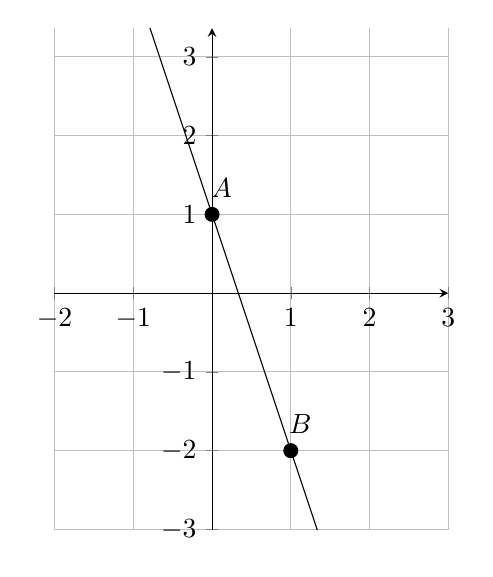
\begin{tikzpicture}[line cap=round,line join=round,>=triangle 45,x=1.0cm,y=1.0cm]
\begin{axis}[
x=1.0cm,y=1.0cm,
axis lines=middle,
ymajorgrids=true,
xmajorgrids=true,
xmin=-2.0,
xmax=3.0,
ymin=-3.0,
ymax=3.3645818181818212,
xtick={-2.0,-1.0,...,3.0},
ytick={-3.0,-2.0,...,3.0},]
\clip(-2.,-3.) rectangle (3.,3.3645818181818212);
\draw [domain=-2.:3.] plot(\x,{(--1.-3.*\x)/1.});
\begin{scriptsize}
\draw [fill=black] (0.,1.) circle (2.5pt);
\draw[color=black] (0.12,1.3373090909090932) node {$A$};
\draw [fill=black] (1.,-2.) circle (2.5pt);
\draw[color=black] (1.12,-1.6626909090909077) node {$B$};
\end{scriptsize}
\end{axis}
\end{tikzpicture}
\end{document}